% subseccion 4.6
\subsection{Etapa 6: Resultados}
Esta sección presenta la información de los resultados obtenidos a través de la ejecución del protocolo de búsqueda SMS. En este sentido, inicialmente se presenta la descripción general de los datos, que corresponden a los SPS. Esta descripción cubre aspectos como el origen de los estudios, año de publicación, la estrategia de búsqueda usada, índices de calidad, la relación de las preguntas de investigación con los tópicos y las palabras claves. Finalmente, se presenta la nube de palabras obtenidad de las palabras claves de los SPS. \\
Es importante recordar que la asociación entre los SPS con los tópicos fue establecido a través de la clasificación de los estudios, como se describe en la sección~\hyperref[sec:clasificacion-estudios]{Clasificación de estudios}. Además, las preguntas de investigación fueron asociadas también de forma inherente debido a que los tópicos tienen una estructura específica dentro de las preguntas de investigación. En este sentido, se identificó la asociación entre las principales palabras claves del SMS con el título del estudio, el resumen y las palabras claves de todos los SPS.
\mbox{}\\

%sub-subseccion 4.6.1
\subsubsection{Descripción General de los SPSs (Estudios Primarios Seleccionados)}
El proceso de búsqueda y selección de estudios, condujo a la identificación de 226 estudios primarios (SPSs), como se observa en la tabla~\ref{tab:sps-list}.
Estos SPS vienen de bases de datos digitales, los cuales se identificaron en el SMS usando diferentes estrategias de búsqueda. La figura~\ref{fig:SPS-BY-SE} muestra el número de estudios identificados a través de diferentes fuentes, detallando la búsqueda en bases de datos y la búsqueda por bola de nieve. En cuanto a la fuente, el 50.88\% de los SPS provienen de la búsqueda por bola de nieve, seguido por el 48.67\% de los SPS que provienen de bases de datos digitales y el 0.44\% de los SPS que provienen de la inclusión directa.
Con respecto a la estrategia de búsqueda en base de datos, la figura~\ref{fig:SPS-BY-SE} muestra que de los 110 SPS identificados a través de esta estrategia, el 86.36\% provienen de IEEE Xplore y ACM Digital Library, el restante 13.64\% se reparte entre las otras fuentes.
En cuanto a la estrategia de búsqueda por bola de nieve, la figura~\ref{fig:SPS-BY-SE} muestra que de los 115 SPS identificados a través de esta estrategia, el 92.17\% provienen de la búsqueda hacia adelante y el 7.82\% restante proviene de la búsqueda hacia atrás.


EXPLICAR FIGURA~\ref{fig:SPS-VBC}
\begin{figure}[htbp]
    \centering
    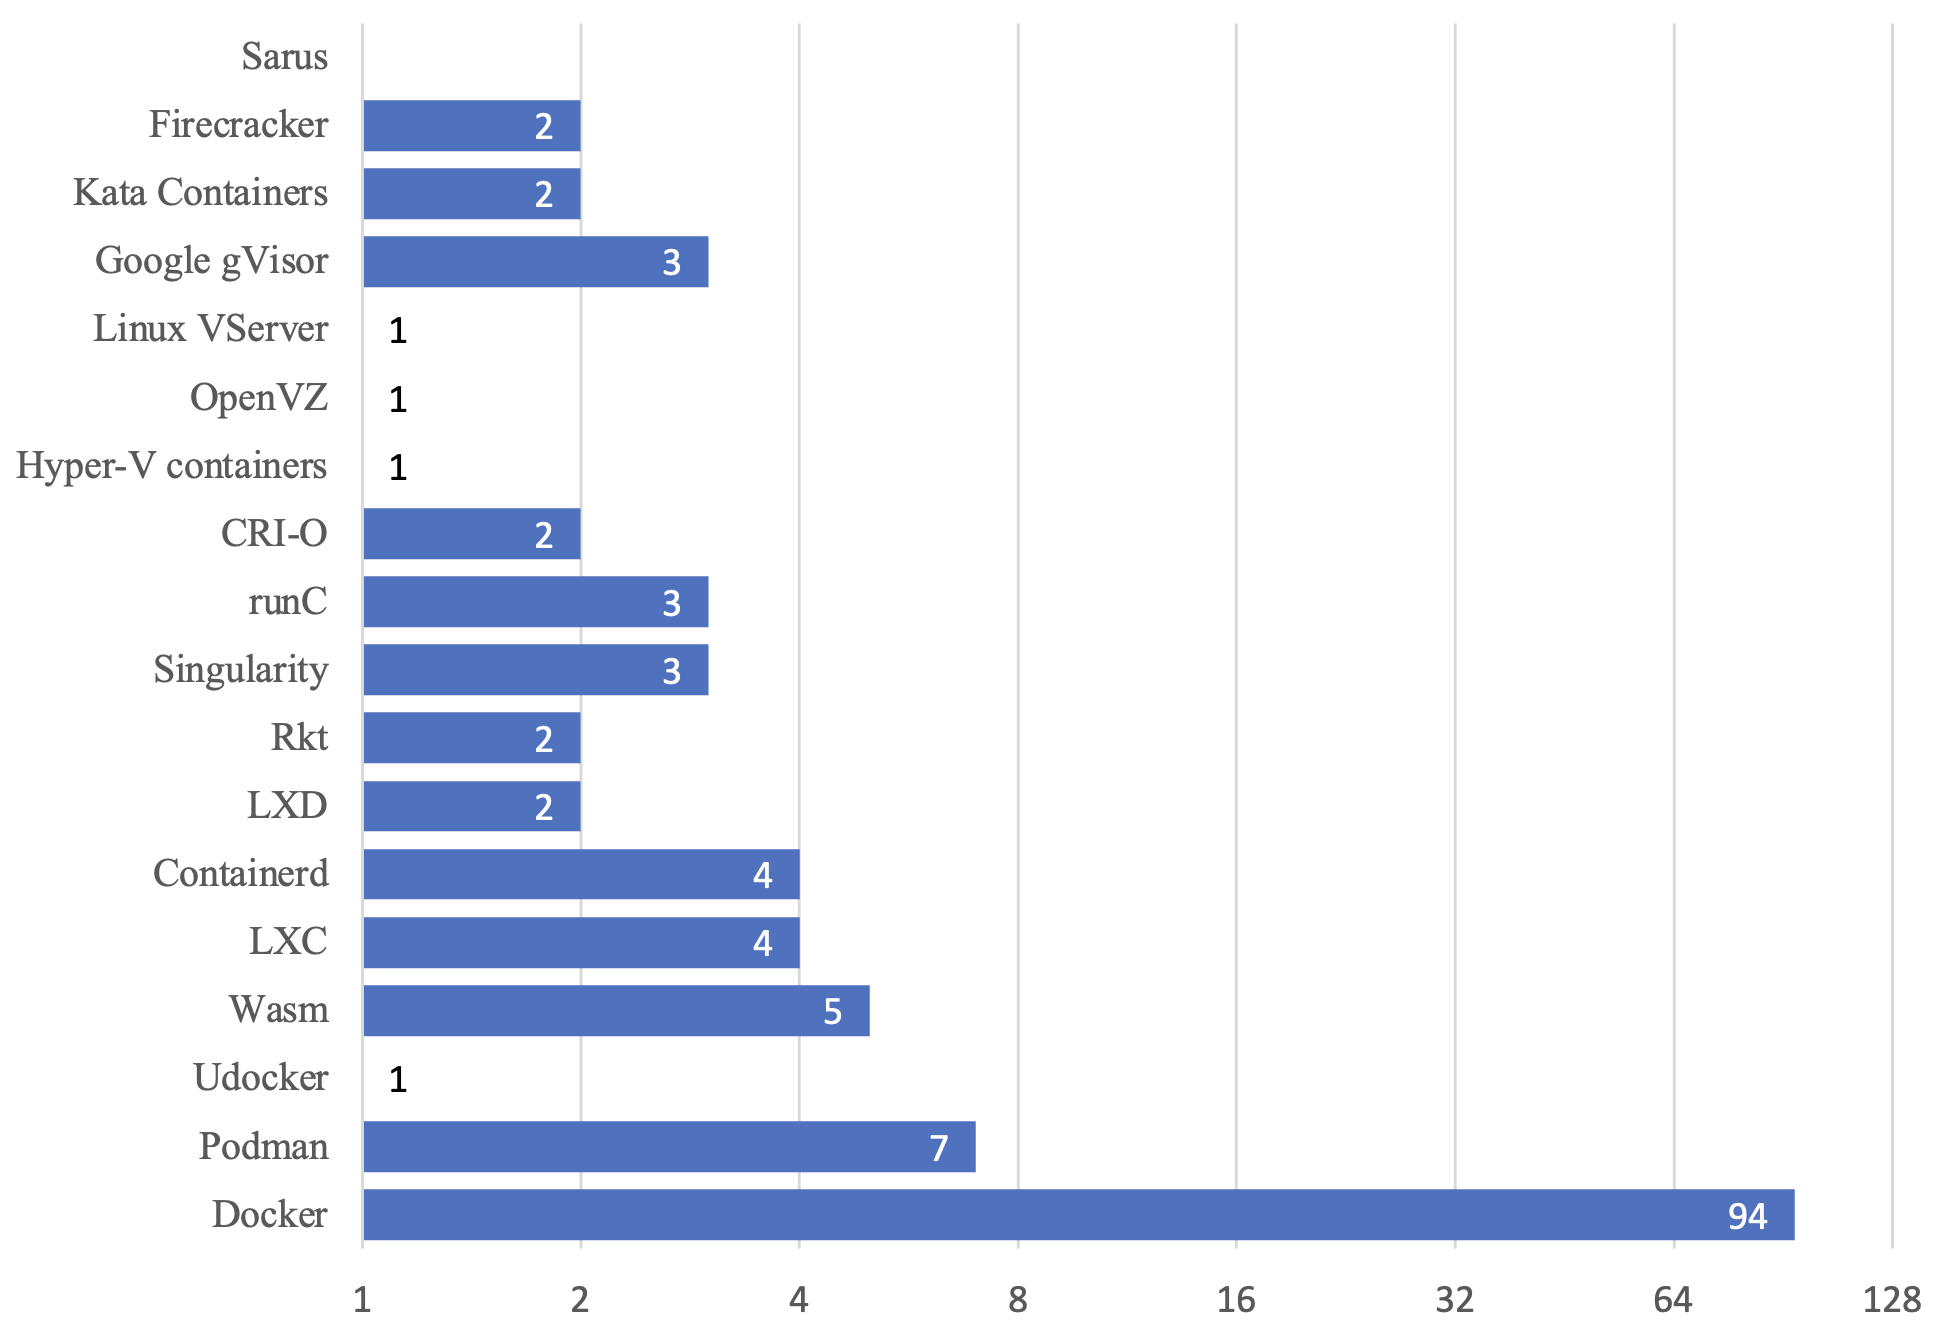
\includegraphics[width=0.5\textwidth]{resources/images/resultados/SPS-VBC.png}
    \caption{Tecnologías de virtualización basadas en contenedores aportadas por cada SPS}\label{fig:SPS-VBC}
\end{figure} 


EXPLICAR FIGURA~\ref{fig:SPS-ORCH}
\begin{figure}[htbp]
    \centering
    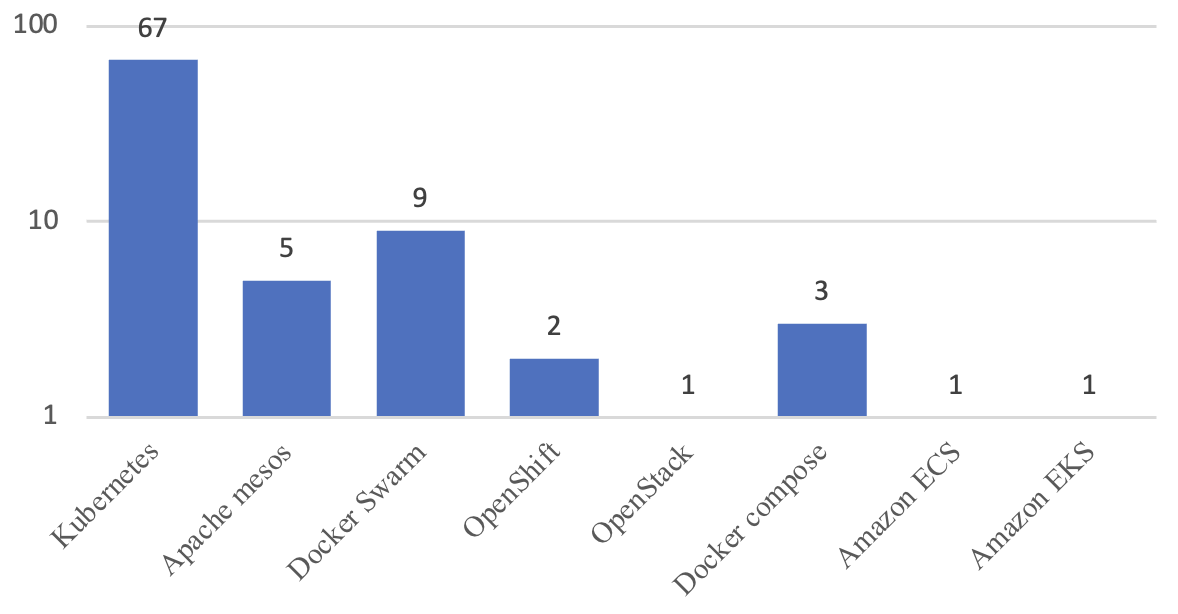
\includegraphics[width=0.5\textwidth]{resources/images/resultados/orch-SPS.png}
    \caption{Tecnologías de orquestadores aportadas por cada SPS}\label{fig:SPS-ORCH}
\end{figure}

EXPLICAR FIGURA~\ref{fig:SPS-venn}
\begin{figure}[htbp]
    \centering
    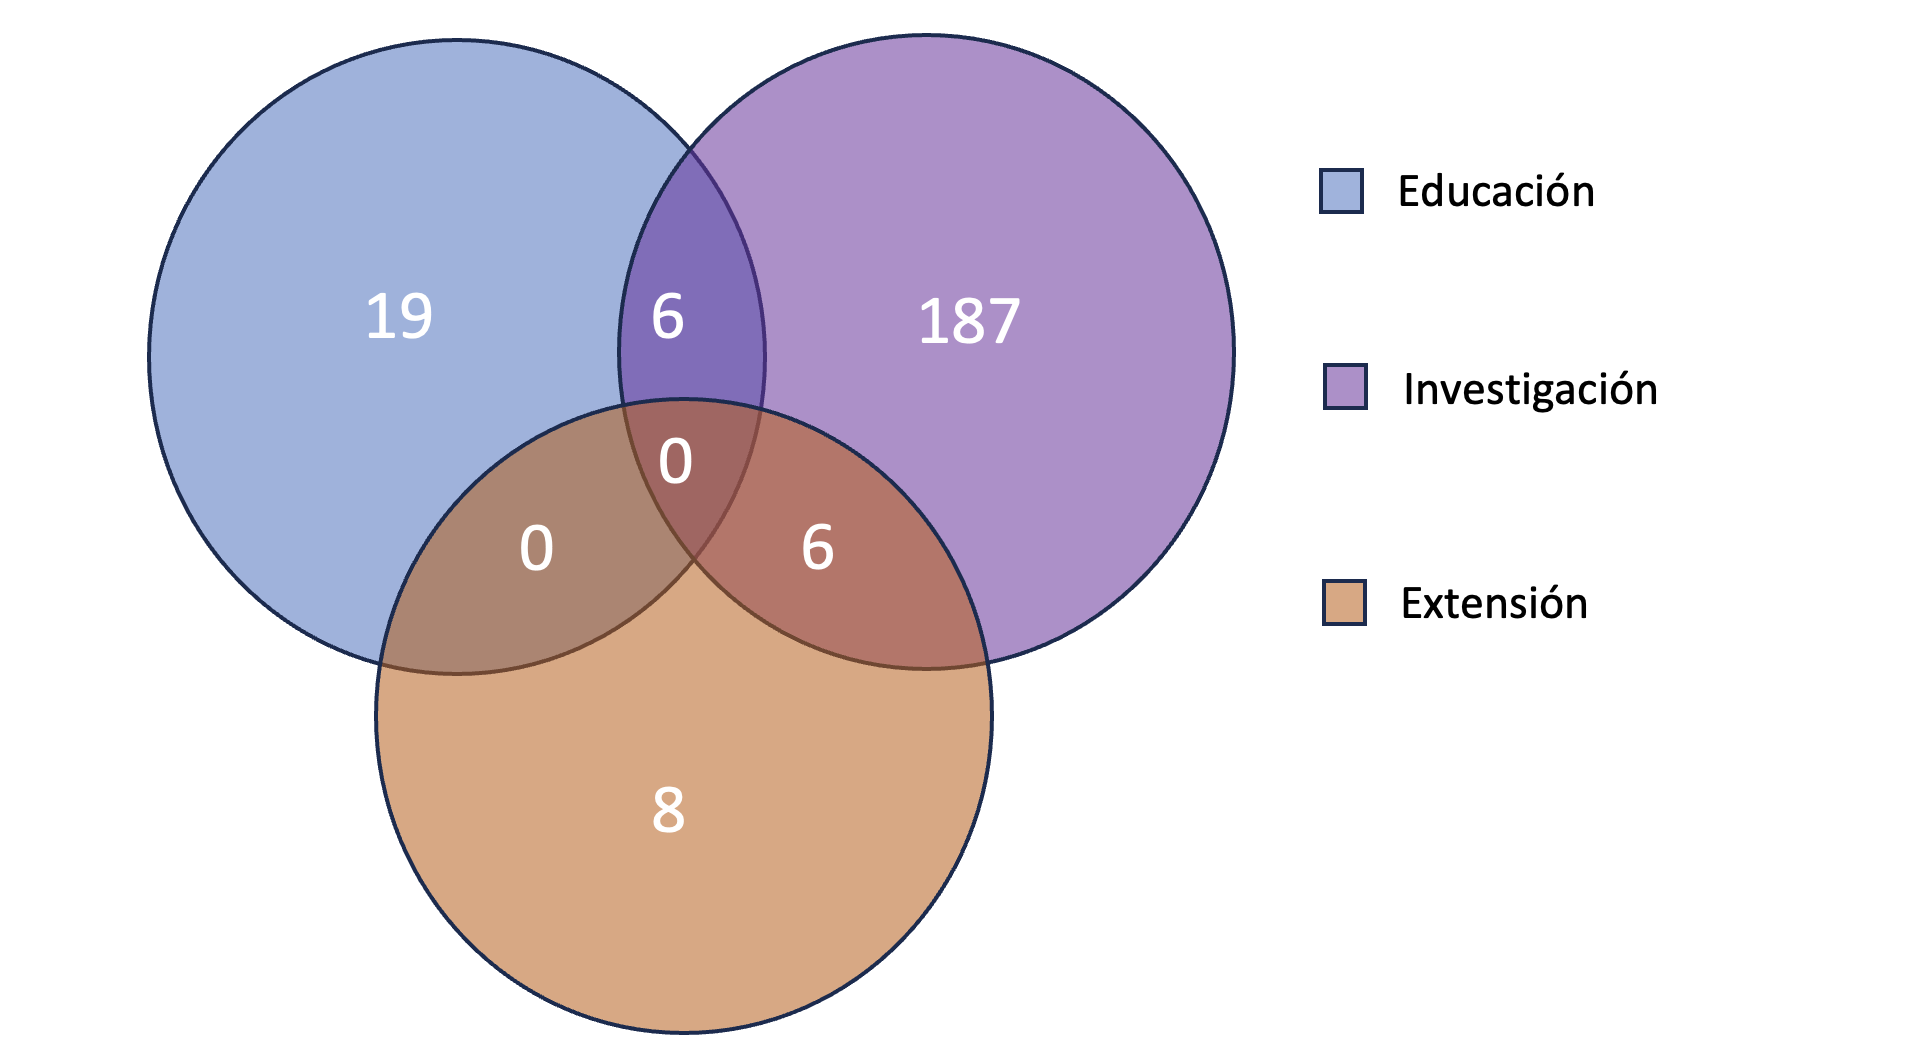
\includegraphics[width=0.5\textwidth]{resources/images/resultados/SPS-venn.png}
    \caption{Diagrama de Venn de los SPS en educación, investigación y extensión}\label{fig:SPS-venn}
\end{figure}

La figura~\ref{fig:SPS-topics} muestra los tópicos definidos en la etapa de planeación para cada pregunta de investigación y el número de SPS relacionados con cada tópico de forma no exclusiva. Es esencial tener en cuenta que un SPS puede estar relacionado a diferentes tópicos simultáneamente. En este sentido, la figura~\ref{fig:SPS-topics} refleja los tres tópicos asociados a la pregunta de investigación 1, de los cuales el tópico ``Investigación'' es el más frecuente con el 83.61\% en contraste con el tópico menos frecuente ``Extensión'' con el 5.88\%.
\begin{figure}[htbp]
    \centering
    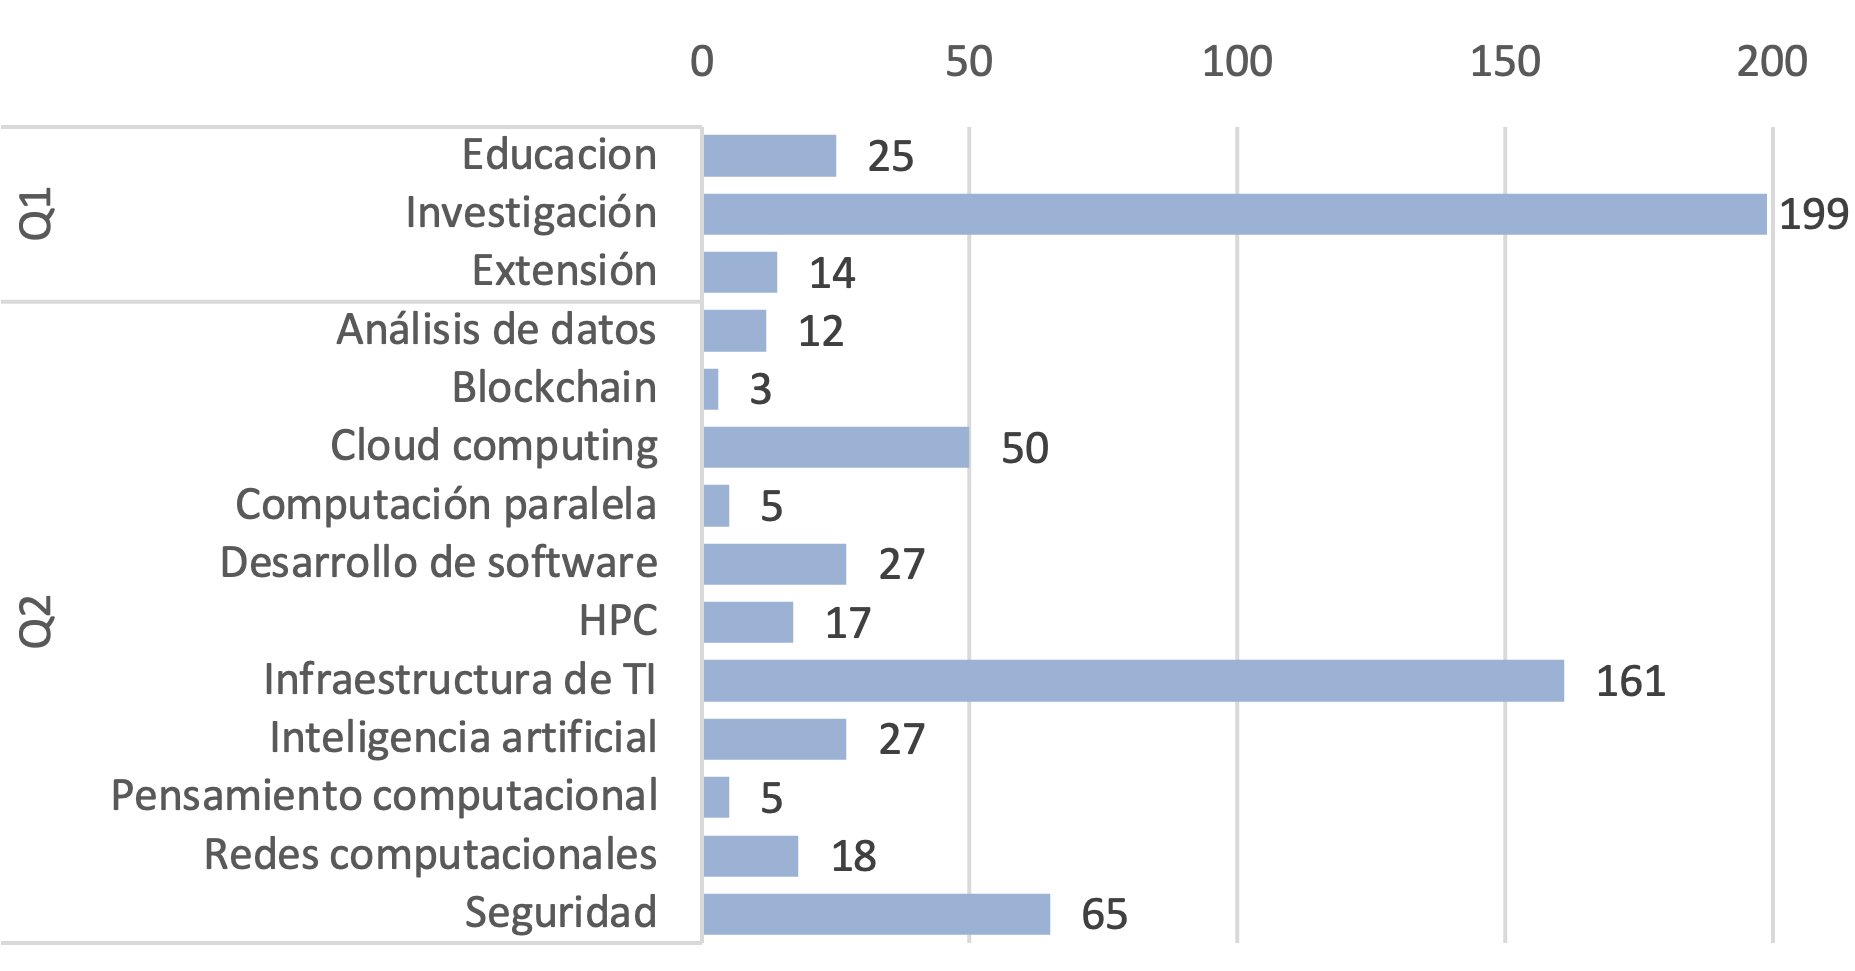
\includegraphics[width=0.5\textwidth]{resources/images/resultados/SPS-topics.png}
    \caption{SPS por preguntas de investigación y tópicos}\label{fig:SPS-topics}
\end{figure}
\mbox{}\\
La figura~\ref{fig:SPS-topics} también muestra los 11 tópicos asociados a la pregunta de investigación 2, en el cual el tópico ``Infraestructura de TI'' es el más frecuente con el  41.28\%. En contraste, el tópico menos frecuente es ``Blockchain'' con el 0.76\%. Considerando que el período de investigación incluye estudios desde el año 2022 hasta el 2024, la figura~\ref{fig:SPS-QI} muestra un crecimiento en el número de SPS publicados desde el 2022, pasando de 30 en 2022 a 107 en 2024. El mayor crecimiento se observa en el 2024, pasando 70 SPS a 109 SPS, un aumento del 55.71\%.\\
\begin{figure}[htbp]
    \centering
    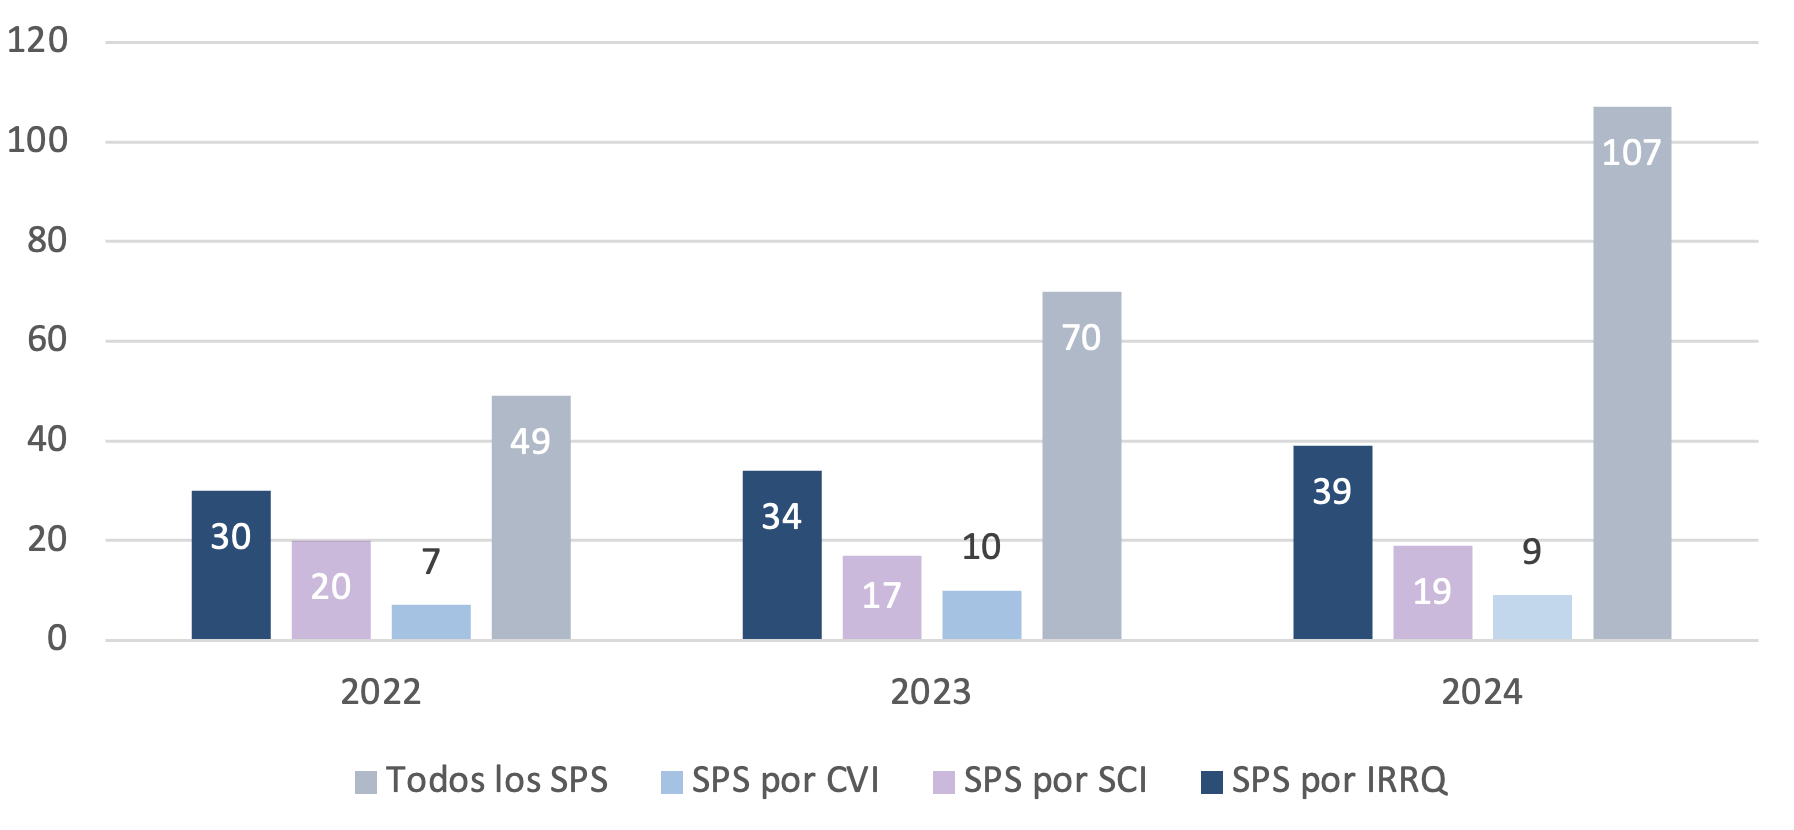
\includegraphics[width=0.5\textwidth]{resources/images/resultados/SPS-by-se.png}
    \caption{SPS por fuente y estrategia de búsqueda en base de datos}\label{fig:SPS-BY-SE}
\end{figure}
De acuerdo con el índice de calidad SCI, este se mantiene relativamente estable y apegado al promedio de 18. Aunque, es importante resaltar una caída del 15\% entre los años 2022 y 2023; sin embargo, en el 2024 se observa un aumento del 11.8\% en comparación con el 2023. Con relación al índice de calidad CVI, se evidencia una tendencia global hacia el aumento, ya que pasa de 7 en 2022 a 9 en 2024 lo que significa un crecimiento neto del 28.6\%. El índice de calidad IRRQ muestra una tendencia sostenida y presenta una baja dispersión con una desviación estándar de 3.68. Además, muestra un crecimiento sostenido en el período 2022 a 2024 pasando de 30 en 2022 a 34 en 2023, representando un incremento del 13.3\%. Posteriormente, en 2024 se observa un aumento del 14.7\% en comparación con el 2023. En el acumulado del período 2022 a 2024, el índice IRRQ pasa de 30 a 39, lo que representa un crecimiento total del 30\%.\\
\begin{figure}[htbp]
    \centering
    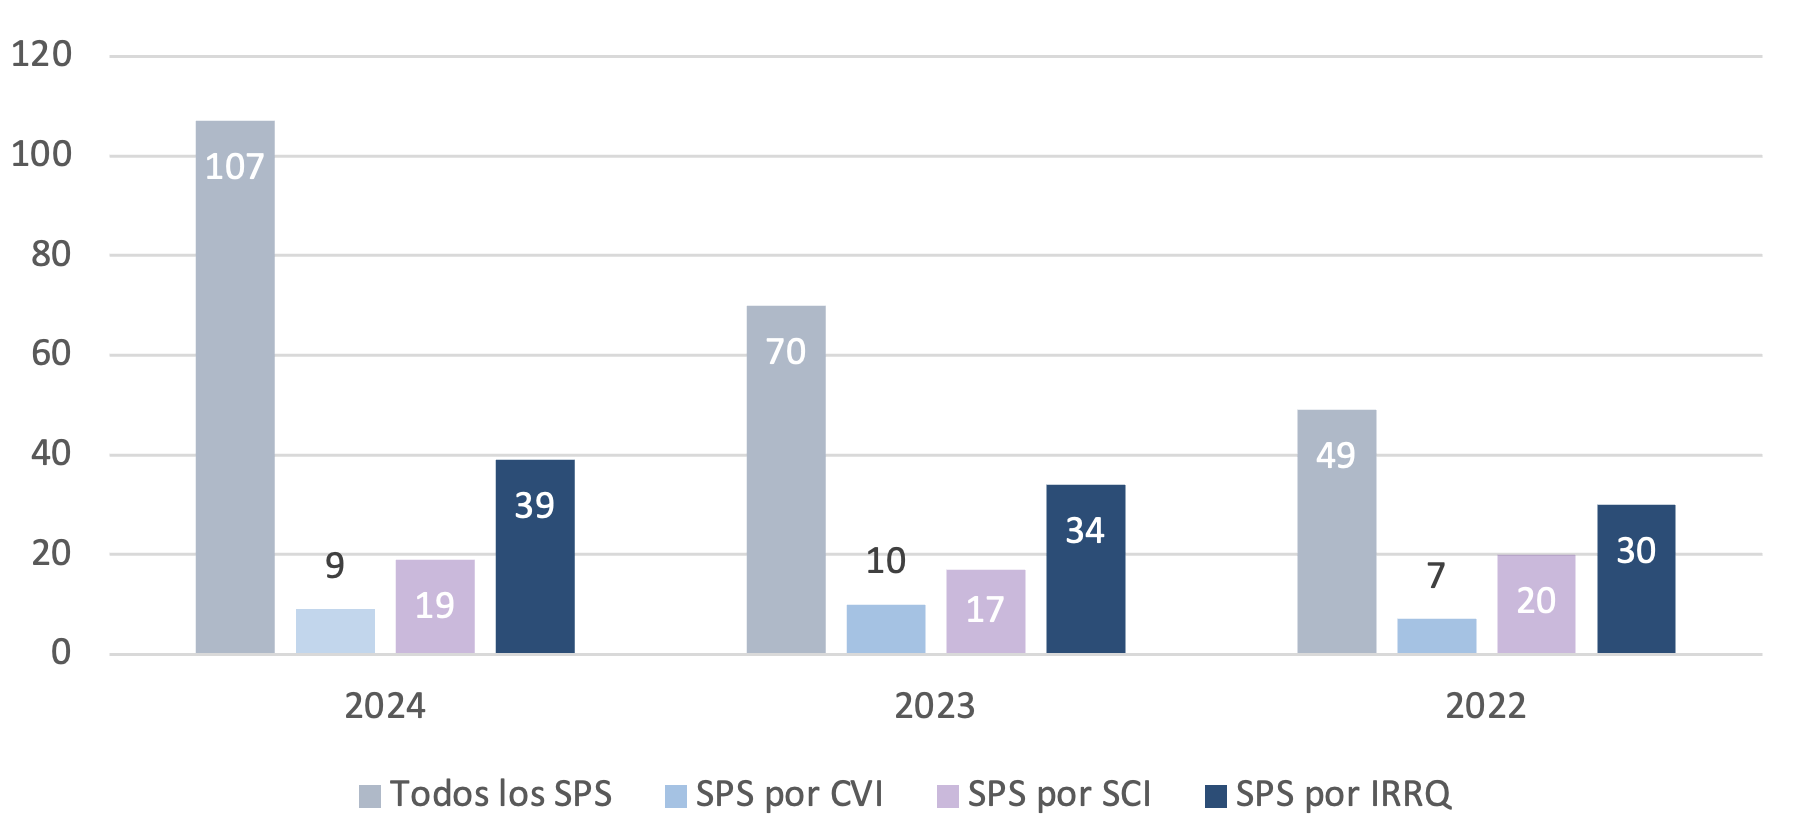
\includegraphics[width=0.5\textwidth]{resources/images/resultados/SPS-QI.png}
    \caption{SPS por año e índices}\label{fig:SPS-QI}
\end{figure}
La figura~\ref{fig:SPS-topics-QI} muestra el número de SPS clasificados de acuerdo a las preguntas de investigación incluidos sus respectivos tópicos, agregando además los índices de calidad. En este sentido, este estudio indica que sobre la pregunta de investigación 1, el tópico extensión es que menos SPS tiene, con un total de 8 SPS, equivalente al 7.33\%. En contraste, el tópico investigación es el que más SPS tiene, con un total de 80 SPS, equivalente al 73.39\%. Para la pregunta de investigación de investigación 2, el tópico Infraestructura de TI es el que más SPS registra, con un total de 73 SPS, equivalente al 43.71\% seguido por el tópico \textit{Cloud Computing} con un total de 24 SPS, equivalente al 14.37\%. 

\begin{figure}[htbp]
    \centering
    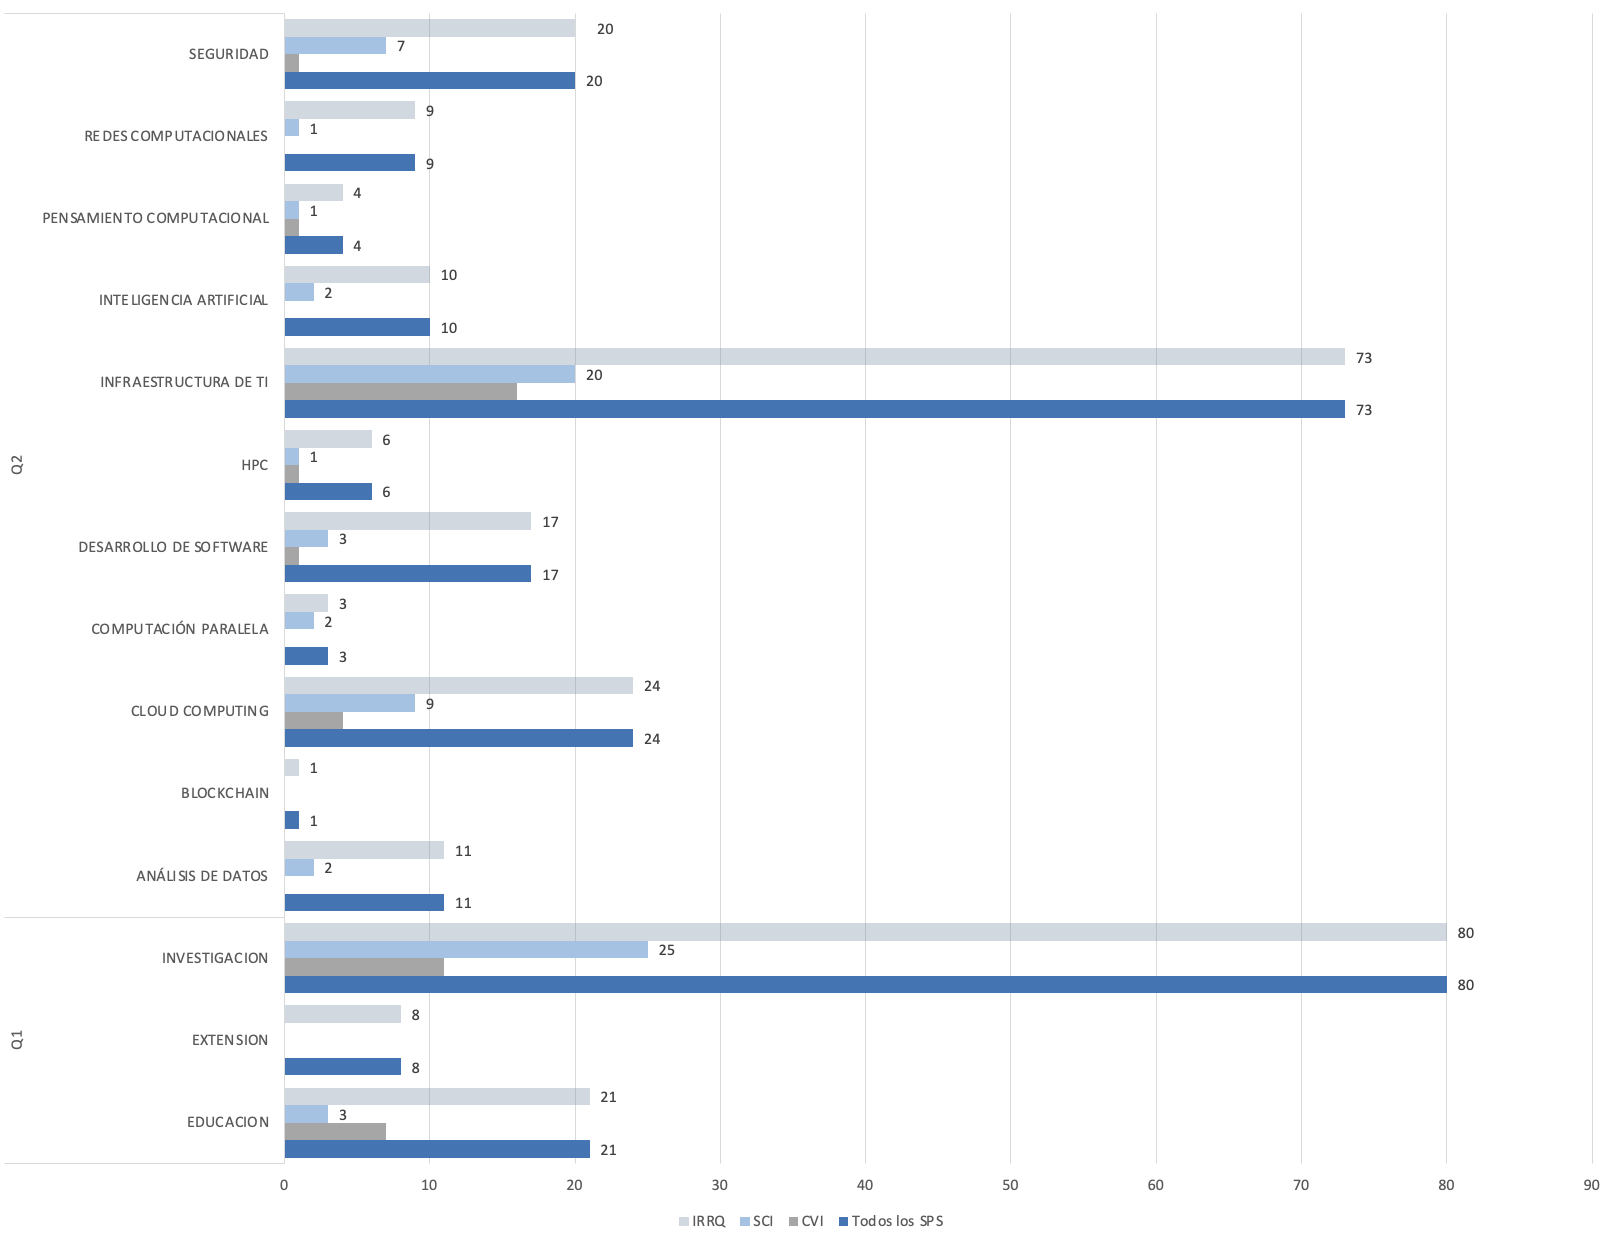
\includegraphics[width=0.5\textwidth]{resources/images/resultados/SPS-topics-QI.png}
    \caption{SPS por índices, tópicos y preguntas de investigación}\label{fig:SPS-topics-QI}
\end{figure}
La figura~\ref{fig:SPS-kw} muestra un cruce entre los SPS, las principales palabras claves y sus sinónimos. Para el contexto de los dominios de TI destaca la palabra clave \textit{Container} que permitió registar un total de 57 SPS. En cuanto al contexto de Educación, Investigación y Extensión se evidencian pocas palabras clave identificadas siendo \textit{Learning} y \textit{Cibersecurity education} las únicas presentes, con un total de 2 SPS cada una. \\
\begin{figure}[htbp]
    \centering
    \includegraphics[width=0.5\textwidth]{resources/images/resultados/Kw.png}
    \caption{SPS por palabras clave}\label{fig:SPS-kw}
\end{figure}
\mbox{}\\
%sub-subseccion 4.6.2
\subsubsection{Visualización de Nube de Palabras}
Otro resultado de obtenido de los 226 SPS es la nube de palabras del mapeo sistemático. Con este tipo de gráfico se identifica el uso de palabras y conceptos que colectivamente tiene mayor frecuencia en el conjunto de los estudios. La figura~\ref{fig:SPS-wordcloud} muestra la nube de palabras generada con una herramienta en línea. Esta herramienta permitió generar la nube de palabras con las palabras claves de los SPS con una frecuencia mayor a 1.
Entre las palabras más frecuentes se encuentran: Docker, \textit{Container}, Kubernetes, \textit{Cloud Computing} que representan el 61.6\% del total de palabras claves. El segundo nivel de palabras claves incluye: \textit{Containerization}, \textit{Container Orchestration}, \textit{virtualization} y \textit{Microservices} que representa el 13.08\%. El tercer nivel está compuesto por las palabras claves: \textit{Performance evaluation}, \textit{Edge computing}, \textit{Machine learning} y \textit{Security} que representa el 9.09\%.
\begin{figure}[htbp]
    \centering
    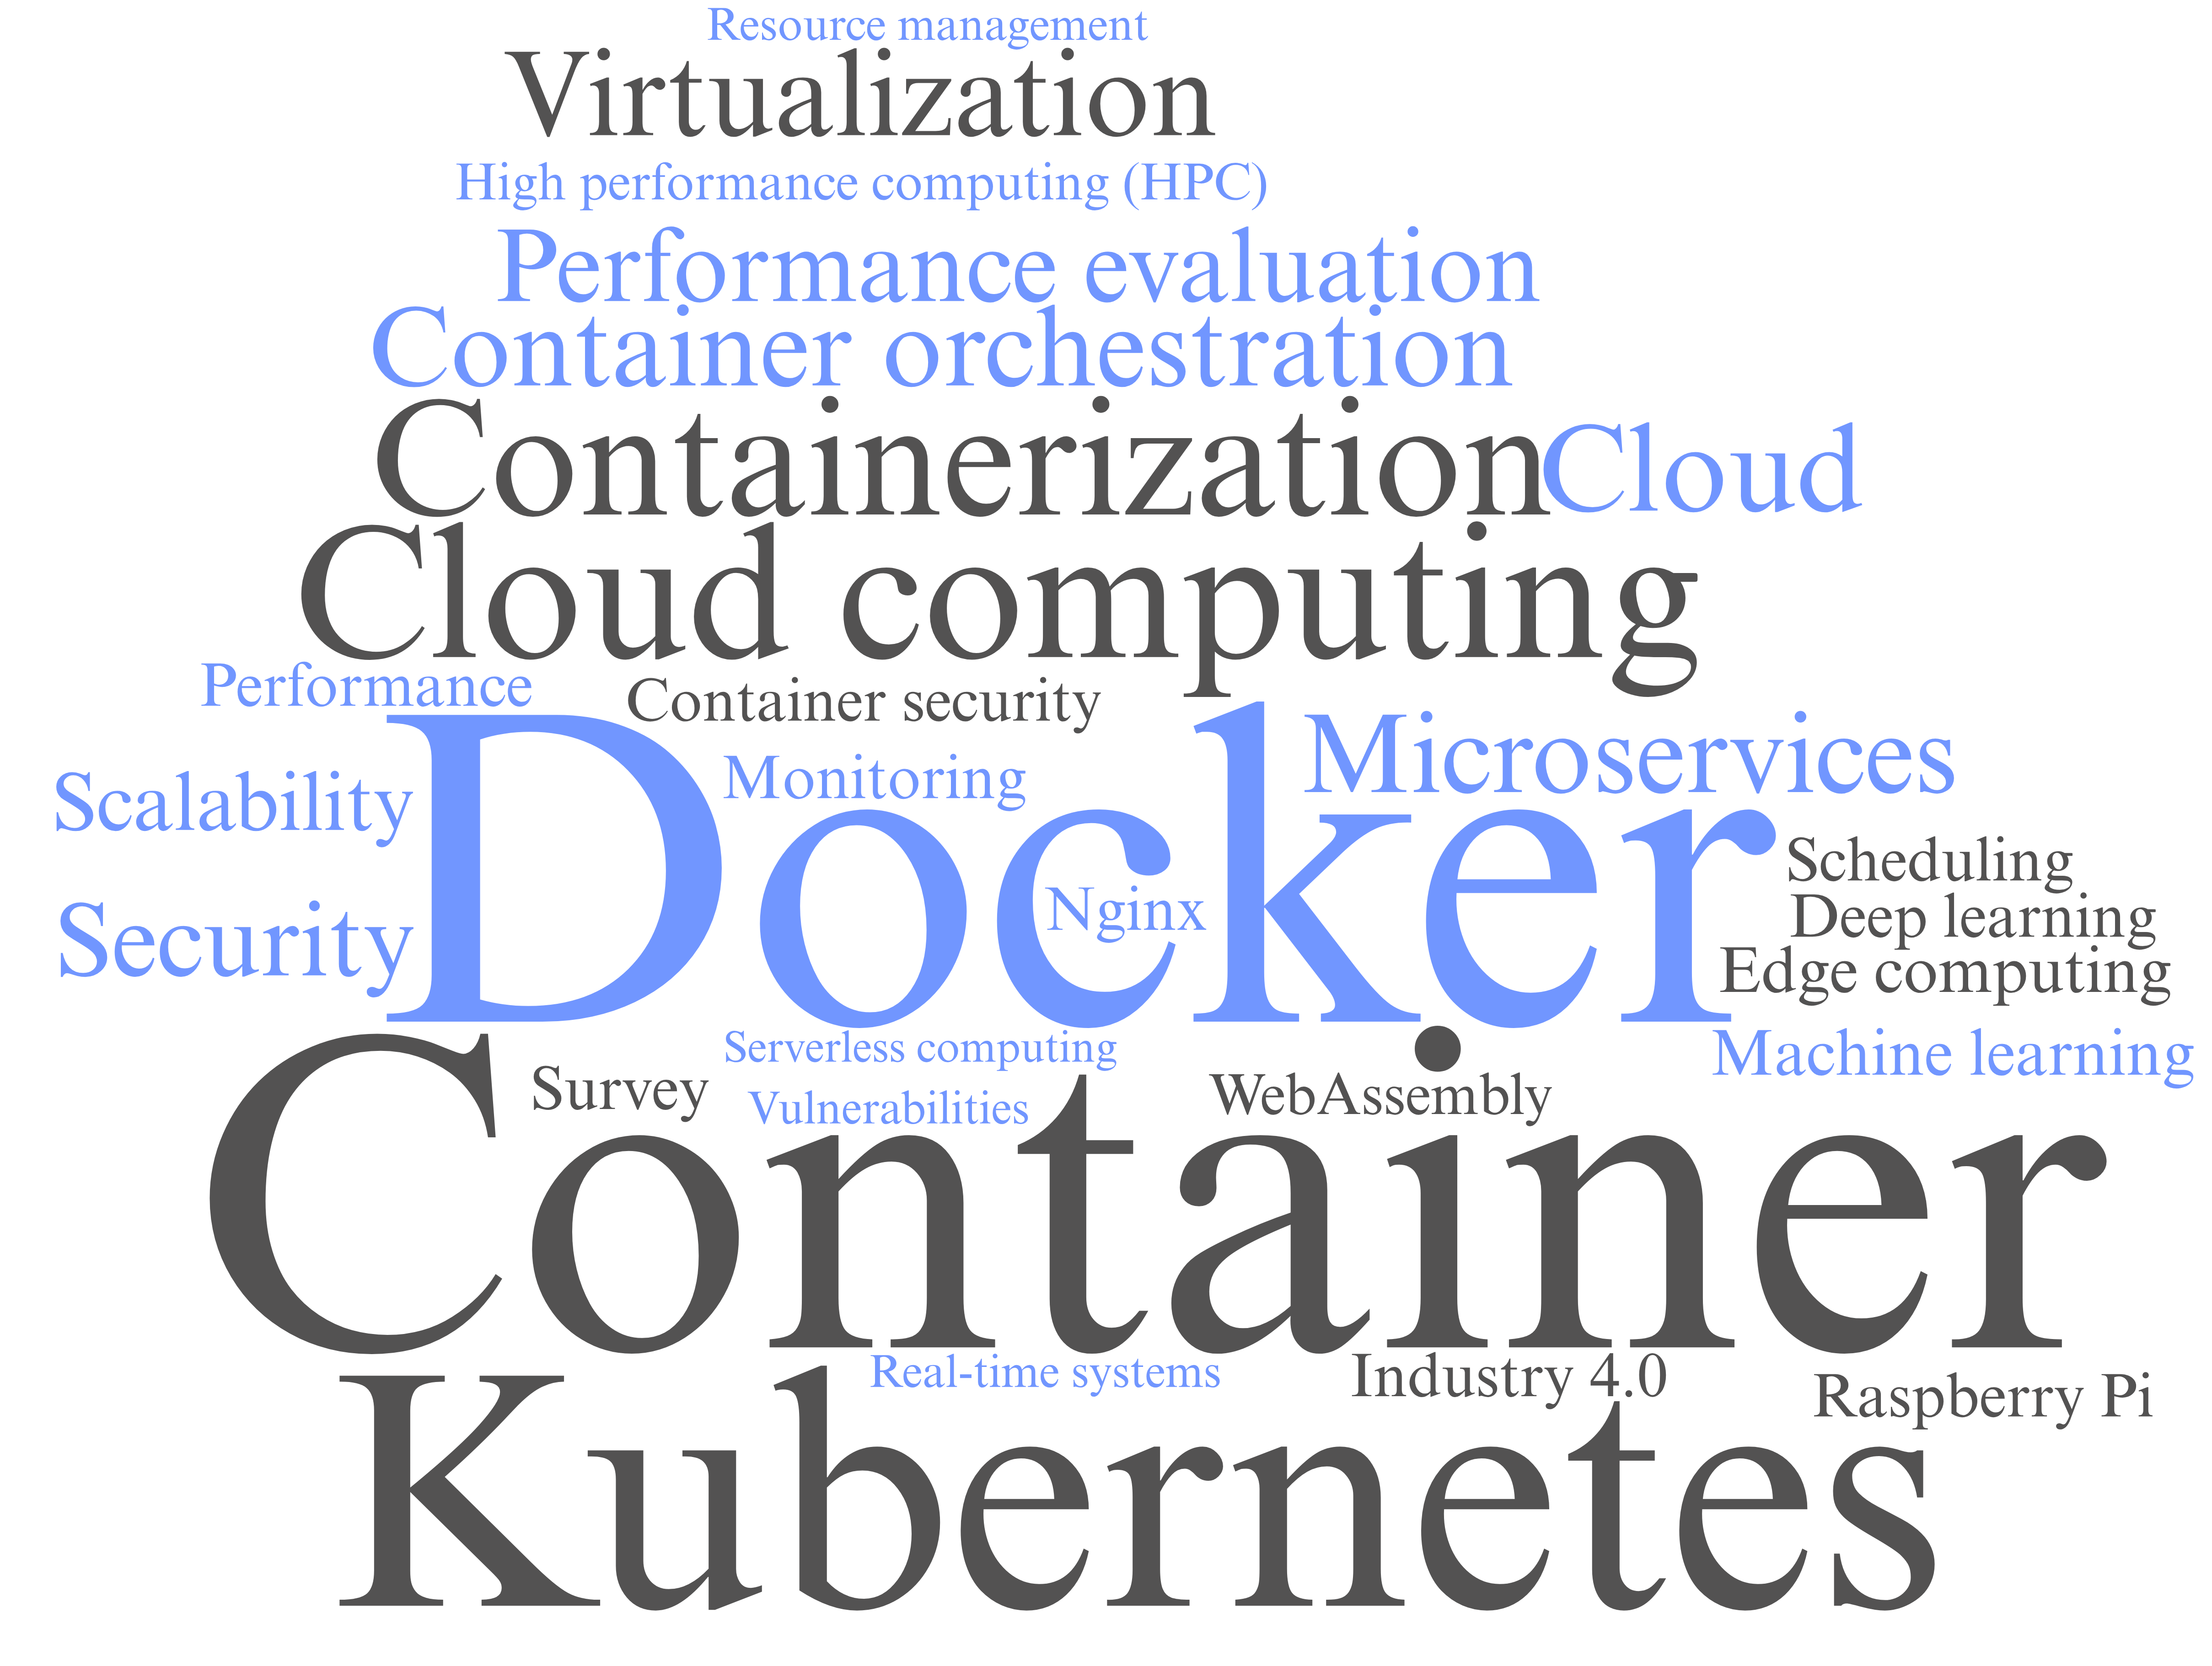
\includegraphics[width=0.5\textwidth]{resources/images/resultados/wordcloud.png}
    \caption{Nube de palabras}\label{fig:SPS-wordcloud}
\end{figure}
\mbox{}\\